\documentclass[twoside]{book}

% Packages required by doxygen
\usepackage{fixltx2e}
\usepackage{calc}
\usepackage{doxygen}
\usepackage[export]{adjustbox} % also loads graphicx
\usepackage{graphicx}
\usepackage[utf8]{inputenc}
\usepackage{makeidx}
\usepackage{multicol}
\usepackage{multirow}
\PassOptionsToPackage{warn}{textcomp}
\usepackage{textcomp}
\usepackage[nointegrals]{wasysym}
\usepackage[table]{xcolor}

% NLS support packages
\usepackage[spanish]{babel}
% Font selection
\usepackage[T1]{fontenc}
\usepackage[scaled=.90]{helvet}
\usepackage{courier}
\usepackage{amssymb}
\usepackage{sectsty}
\renewcommand{\familydefault}{\sfdefault}
\allsectionsfont{%
  \fontseries{bc}\selectfont%
  \color{darkgray}%
}
\renewcommand{\DoxyLabelFont}{%
  \fontseries{bc}\selectfont%
  \color{darkgray}%
}
\newcommand{\+}{\discretionary{\mbox{\scriptsize$\hookleftarrow$}}{}{}}

% Page & text layout
\usepackage{geometry}
\geometry{%
  a4paper,%
  top=2.5cm,%
  bottom=2.5cm,%
  left=2.5cm,%
  right=2.5cm%
}
\tolerance=750
\hfuzz=15pt
\hbadness=750
\setlength{\emergencystretch}{15pt}
\setlength{\parindent}{0cm}
\setlength{\parskip}{3ex plus 2ex minus 2ex}
\makeatletter
\renewcommand{\paragraph}{%
  \@startsection{paragraph}{4}{0ex}{-1.0ex}{1.0ex}{%
    \normalfont\normalsize\bfseries\SS@parafont%
  }%
}
\renewcommand{\subparagraph}{%
  \@startsection{subparagraph}{5}{0ex}{-1.0ex}{1.0ex}{%
    \normalfont\normalsize\bfseries\SS@subparafont%
  }%
}
\makeatother

% Headers & footers
\usepackage{fancyhdr}
\pagestyle{fancyplain}
\fancyhead[LE]{\fancyplain{}{\bfseries\thepage}}
\fancyhead[CE]{\fancyplain{}{}}
\fancyhead[RE]{\fancyplain{}{\bfseries\leftmark}}
\fancyhead[LO]{\fancyplain{}{\bfseries\rightmark}}
\fancyhead[CO]{\fancyplain{}{}}
\fancyhead[RO]{\fancyplain{}{\bfseries\thepage}}
\fancyfoot[LE]{\fancyplain{}{}}
\fancyfoot[CE]{\fancyplain{}{}}
\fancyfoot[RE]{\fancyplain{}{\bfseries\scriptsize Generado por Doxygen }}
\fancyfoot[LO]{\fancyplain{}{\bfseries\scriptsize Generado por Doxygen }}
\fancyfoot[CO]{\fancyplain{}{}}
\fancyfoot[RO]{\fancyplain{}{}}
\renewcommand{\footrulewidth}{0.4pt}
\renewcommand{\chaptermark}[1]{%
  \markboth{#1}{}%
}
\renewcommand{\sectionmark}[1]{%
  \markright{\thesection\ #1}%
}

% Indices & bibliography
\usepackage{natbib}
\usepackage[titles]{tocloft}
\setcounter{tocdepth}{3}
\setcounter{secnumdepth}{5}
\makeindex

% Hyperlinks (required, but should be loaded last)
\usepackage{ifpdf}
\ifpdf
  \usepackage[pdftex,pagebackref=true]{hyperref}
\else
  \usepackage[ps2pdf,pagebackref=true]{hyperref}
\fi
\hypersetup{%
  colorlinks=true,%
  linkcolor=blue,%
  citecolor=blue,%
  unicode%
}

% Custom commands
\newcommand{\clearemptydoublepage}{%
  \newpage{\pagestyle{empty}\cleardoublepage}%
}

\usepackage{caption}
\captionsetup{labelsep=space,justification=centering,font={bf},singlelinecheck=off,skip=4pt,position=top}

%===== C O N T E N T S =====

\begin{document}

% Titlepage & ToC
\hypersetup{pageanchor=false,
             bookmarksnumbered=true,
             pdfencoding=unicode
            }
\pagenumbering{alph}
\begin{titlepage}
\vspace*{7cm}
\begin{center}%
{\Large Turtle -\/ opengl }\\
\vspace*{1cm}
{\large Generado por Doxygen 1.8.13}\\
\end{center}
\end{titlepage}
\clearemptydoublepage
\pagenumbering{roman}
\tableofcontents
\clearemptydoublepage
\pagenumbering{arabic}
\hypersetup{pageanchor=true}

%--- Begin generated contents ---
\chapter{Página principal}
\label{index}\hypertarget{index}{}El codigo esta estructurado para que se use como la tortuga original de python. el algoritmo usa calculos matematicos basicos. 
\chapter{Turtle open\+GL}
\label{md_README}
\Hypertarget{md_README}
\subsection*{Description}

Implementation of python turtle in Opengl c++

\subsection*{Compile}

\subsubsection*{Install glut(\+Ubuntu)\+:}

\begin{DoxyVerb}sudo apt install build-essential ubuntu-restricted-extras cimg-dev freeglut3-dev libgles2-mesa-dev
sudo apt install g++
sudo apt-get install freeglut3-dev
\end{DoxyVerb}


\subsubsection*{Finally execute\+:}

\begin{DoxyVerb}g++ main.cpp plano.cpp -o gl -lGL -lGLU -lglut
./gl
\end{DoxyVerb}


\#\# Struct of the coordenadas 
\begin{DoxyCode}
\{c++\}
struct coordenada\{
    t\_coord x,y;
    int R,G,B;
    t\_coord grados;
\};
\end{DoxyCode}


\subsection*{Struct of the plano}


\begin{DoxyCode}
\{c++\}
class plano\{
    private:
    coordenada pla;
    t\_coord xini,yini;
    int h,w;
    \}
\end{DoxyCode}
 \subsection*{Rotate}


\begin{DoxyItemize}
\item Calculate new coordinates with\+: 
\begin{DoxyCode}
y = y + (tam * sin(grados));
x = x + (tam * cos(grados));
\end{DoxyCode}
 \subsection*{Authors}
\end{DoxyItemize}


\begin{DoxyItemize}
\item \href{https://github.com/walker1239}{\tt Walker Fernando Manrique Chalco} 
\end{DoxyItemize}
\chapter{Índice de clases}
\section{Lista de clases}
Lista de las clases, estructuras, uniones e interfaces con una breve descripción\+:\begin{DoxyCompactList}
\item\contentsline{section}{\hyperlink{classAbstractFactory}{Abstract\+Factory} \\*La clase \hyperlink{classAbstractFactory}{Abstract\+Factory} contiene funciones para crear todo el paint  Se instancia el dato miembro }{\pageref{classAbstractFactory}}{}
\item\contentsline{section}{\hyperlink{classarbol}{arbol} \\*La clase arbol contiene la funcion drawn para visualizar el arbol  Se instancia los datos miembros que son punteros a las partes del arbol }{\pageref{classarbol}}{}
\item\contentsline{section}{\hyperlink{classarbol__normal}{arbol\+\_\+normal} \\*La clase \hyperlink{classarbol__normal}{arbol\+\_\+normal} hereda del arbol, estes es un arbol normal y unico. Tambien puede ser modificado.  Las funciones apuntan a las clases de las partes del arbol, asi como tambien son void }{\pageref{classarbol__normal}}{}
\item\contentsline{section}{\hyperlink{classbuilder}{builder} \\*La clase builder contiene las funciones gettronco, gethojas, getramas para obtener las caracteristicas del arbol en sus clases hijas  Las funciones son virtual-\/puras y apuntan a las clases de las partes del arbol }{\pageref{classbuilder}}{}
\item\contentsline{section}{\hyperlink{structcoordenada}{coordenada} }{\pageref{structcoordenada}}{}
\item\contentsline{section}{\hyperlink{classdirector}{director} \\*La clase director es la que crea mediante el builder o mediante parametros }{\pageref{classdirector}}{}
\item\contentsline{section}{\hyperlink{classflor}{flor} \\*La clase flor contiene la funcion drawn para poder dibujarlo en pantalla  Se instancia el dato miembro }{\pageref{classflor}}{}
\item\contentsline{section}{\hyperlink{classflor__bonita}{flor\+\_\+bonita} \\*La clase \hyperlink{classflor__bonita}{flor\+\_\+bonita} es un tipo de flor en la que su dibujo es bonito,contiene la funcion drawn para poder visualizarlo, hereda de la clase flor  Se tiene constructor y destructor }{\pageref{classflor__bonita}}{}
\item\contentsline{section}{\hyperlink{classflor__fea}{flor\+\_\+fea} \\*La clase \hyperlink{classflor__fea}{flor\+\_\+fea} es un tipo de flor en la que su dibujo es feo,contiene la funcion drawn para poder visualizarlo, hereda de la clase flor  Se instancia el dato miembro }{\pageref{classflor__fea}}{}
\item\contentsline{section}{\hyperlink{classflor__regular}{flor\+\_\+regular} \\*La clase \hyperlink{classflor__regular}{flor\+\_\+regular} es un tipo de flor en la que su dibujo es \hyperlink{classflor__regular}{flor\+\_\+regular},contiene la funcion drawn para poder visualizarlo, hereda de la clase flor  Se instancia el dato miembro }{\pageref{classflor__regular}}{}
\item\contentsline{section}{\hyperlink{classhoja}{hoja} \\*La clase hoja contiene la funcion drawn para poder dibujará  Se instancia el dato miembro }{\pageref{classhoja}}{}
\item\contentsline{section}{\hyperlink{classnieve}{nieve} \\*La clase nieve es la clase que crea las particulas de nieve.  Se instancia el dato miembro }{\pageref{classnieve}}{}
\item\contentsline{section}{\hyperlink{classpaint1}{paint1} \\*La clase \hyperlink{classpaint1}{paint1} es un tipo de paint que tiene a arboles y a flores y tambien niev  Se instancia el dato miembro }{\pageref{classpaint1}}{}
\item\contentsline{section}{\hyperlink{classpaint2}{paint2} \\*La clase \hyperlink{classpaint2}{paint2} es un tipo de paint que tiene a arboles y a flores y tambien nieve  Se instancia el dato miembro }{\pageref{classpaint2}}{}
\item\contentsline{section}{\hyperlink{classparticles}{particles} \\*La clase particles es la calse que dibuja solo una particula.  Se instancia el dato miembro }{\pageref{classparticles}}{}
\item\contentsline{section}{\hyperlink{classplano}{plano} \\*La clase plano tiene los elementos basicos para empezar a dibujar como se hace en la python turtle.  Definicion de la funciones usadas en la clase }{\pageref{classplano}}{}
\item\contentsline{section}{\hyperlink{classrama}{rama} \\*La clase rama contiene la funcion drawn para poder dibujará.  Se instancia el dato miembro }{\pageref{classrama}}{}
\item\contentsline{section}{\hyperlink{classsnow__flyweight}{snow\+\_\+flyweight} \\*La clase \hyperlink{classsnow__flyweight}{snow\+\_\+flyweight} es el singleton que dibuja la nieve.  Se instancia el dato miembro }{\pageref{classsnow__flyweight}}{}
\item\contentsline{section}{\hyperlink{classtronco}{tronco} \\*La clase tronco contiene la funcion drawn para poder dibujarlo  Se instancia el dato miembro }{\pageref{classtronco}}{}
\end{DoxyCompactList}

\chapter{Indice de archivos}
\section{Lista de archivos}
Lista de todos los archivos documentados y con descripciones breves\+:\begin{DoxyCompactList}
\item\contentsline{section}{\hyperlink{Abstract_8cpp}{Abstract.\+cpp} \\*Implementacion de la clase paints para la creacion de paints en Glut Open\+GL }{\pageref{Abstract_8cpp}}{}
\item\contentsline{section}{\hyperlink{Abstract_8h}{Abstract.\+h} \\*Implementacion de la clase paints para la creacion de paints en Glut Open\+GL }{\pageref{Abstract_8h}}{}
\item\contentsline{section}{\hyperlink{builder__arbol_8cpp}{builder\+\_\+arbol.\+cpp} \\*Implementacion de la clase arbol para la creacion de arboles en Glut Open\+GL }{\pageref{builder__arbol_8cpp}}{}
\item\contentsline{section}{\hyperlink{builder__arbol_8h}{builder\+\_\+arbol.\+h} \\*Implementacion de la clase arbol para la creacion de arboles en Glut Open\+GL }{\pageref{builder__arbol_8h}}{}
\item\contentsline{section}{\hyperlink{factory__method__flor_8cpp}{factory\+\_\+method\+\_\+flor.\+cpp} \\*Implementacion de la clase flor para la creacion de flores en Glut Open\+GL }{\pageref{factory__method__flor_8cpp}}{}
\item\contentsline{section}{\hyperlink{factory__method__flor_8h}{factory\+\_\+method\+\_\+flor.\+h} \\*Implementacion de la clase flor para la creacion de flores en Glut Open\+GL }{\pageref{factory__method__flor_8h}}{}
\item\contentsline{section}{\hyperlink{flyweight__nieve_8cpp}{flyweight\+\_\+nieve.\+cpp} \\*Implementacion de la clase paints para la creacion de paints en Glut Open\+GL }{\pageref{flyweight__nieve_8cpp}}{}
\item\contentsline{section}{\hyperlink{flyweight__nieve_8h}{flyweight\+\_\+nieve.\+h} \\*Implementacion de la clase paints para la creacion de paints en Glut Open\+GL }{\pageref{flyweight__nieve_8h}}{}
\item\contentsline{section}{\hyperlink{plano_8cpp}{plano.\+cpp} \\*Implementacion de clase plano que permite hacer dibujos usando open\+GL }{\pageref{plano_8cpp}}{}
\item\contentsline{section}{\hyperlink{plano_8h}{plano.\+h} \\*Implementacion de clase plano que permite hacer dibujos usando open\+GL }{\pageref{plano_8h}}{}
\end{DoxyCompactList}

\chapter{Documentación de las clases}
\hypertarget{structcoordenada}{}\section{Referencia de la Estructura coordenada}
\label{structcoordenada}\index{coordenada@{coordenada}}
\subsection*{Atributos públicos}
\begin{DoxyCompactItemize}
\item 
\mbox{\Hypertarget{structcoordenada_a58f4bd357e0e907cc46bcd35f5271e8e}\label{structcoordenada_a58f4bd357e0e907cc46bcd35f5271e8e}} 
t\+\_\+coord {\bfseries x}
\item 
\mbox{\Hypertarget{structcoordenada_a0048d987a8afd0cf94b8ec4a155fcad5}\label{structcoordenada_a0048d987a8afd0cf94b8ec4a155fcad5}} 
t\+\_\+coord {\bfseries y}
\item 
\mbox{\Hypertarget{structcoordenada_a379001d7331a9ecd1b85521e6c1162d3}\label{structcoordenada_a379001d7331a9ecd1b85521e6c1162d3}} 
int {\bfseries R}
\item 
\mbox{\Hypertarget{structcoordenada_a69897a5bd2f9713376d0dc541fd96de2}\label{structcoordenada_a69897a5bd2f9713376d0dc541fd96de2}} 
int {\bfseries G}
\item 
\mbox{\Hypertarget{structcoordenada_ad39661406d2665ff1efe3c695e81a933}\label{structcoordenada_ad39661406d2665ff1efe3c695e81a933}} 
int {\bfseries B}
\item 
\mbox{\Hypertarget{structcoordenada_a35322c013bfbef19997d61111767446f}\label{structcoordenada_a35322c013bfbef19997d61111767446f}} 
t\+\_\+coord {\bfseries grados}
\end{DoxyCompactItemize}


La documentación para esta estructura fue generada a partir del siguiente fichero\+:\begin{DoxyCompactItemize}
\item 
\hyperlink{plano_8h}{plano.\+h}\end{DoxyCompactItemize}

\hypertarget{classplano}{}\section{Referencia de la Clase plano}
\label{classplano}\index{plano@{plano}}


La clase plano tiene los elementos basicos para empezar a dibujar como se hace en la python turtle.  Definicion de la funciones usadas en la clase.  




{\ttfamily \#include $<$plano.\+h$>$}

\subsection*{Métodos públicos}
\begin{DoxyCompactItemize}
\item 
\hyperlink{classplano_a07a6173550219cbe2d32925afac542a5}{plano} (int width=500, int height=500)
\item 
void \hyperlink{classplano_a2febab8f233098b881ced3f4553526f2}{forward} (int cantidad)
\item 
void \hyperlink{classplano_ad5f11338792271b961051f7eff80c4cc}{left} (t\+\_\+coord grado)
\item 
void \hyperlink{classplano_a350bd814b14e4a876b601e608c4b7217}{right} (t\+\_\+coord grado)
\item 
void \hyperlink{classplano_a5758a4e96e2140941dd150e91e6029fd}{set\+\_\+color} (int R, int G, int B)
\item 
void \hyperlink{classplano_a48e4fbc9361ecaffe8a18545825ae19b}{penup} ()
\item 
void \hyperlink{classplano_aa2ae0a48000f85adfc61663ae7011aa2}{pendow} ()
\item 
void \hyperlink{classplano_a87e7fce6efc52d9b8c1e0c8946b1c2bb}{move} (t\+\_\+coord x, t\+\_\+coord y)
\item 
void \hyperlink{classplano_aa17e44a9925d265425e883f3bd8c1565}{display} (int argc, char $\ast$$\ast$argv)
\end{DoxyCompactItemize}


\subsection{Descripción detallada}
La clase plano tiene los elementos basicos para empezar a dibujar como se hace en la python turtle.  Definicion de la funciones usadas en la clase. 

\subsection{Documentación del constructor y destructor}
\mbox{\Hypertarget{classplano_a07a6173550219cbe2d32925afac542a5}\label{classplano_a07a6173550219cbe2d32925afac542a5}} 
\index{plano@{plano}!plano@{plano}}
\index{plano@{plano}!plano@{plano}}
\subsubsection{\texorpdfstring{plano()}{plano()}}
{\footnotesize\ttfamily plano\+::plano (\begin{DoxyParamCaption}\item[{int}]{width = {\ttfamily 500},  }\item[{int}]{height = {\ttfamily 500} }\end{DoxyParamCaption})}

Crear la turtle. por defecto se crea con w1=500 y h 
\begin{DoxyParams}{Parámetros}
{\em width,height} & coordinan el tamano del plano en el que se dibujara. \\
\hline
\end{DoxyParams}


\subsection{Documentación de las funciones miembro}
\mbox{\Hypertarget{classplano_aa17e44a9925d265425e883f3bd8c1565}\label{classplano_aa17e44a9925d265425e883f3bd8c1565}} 
\index{plano@{plano}!display@{display}}
\index{display@{display}!plano@{plano}}
\subsubsection{\texorpdfstring{display()}{display()}}
{\footnotesize\ttfamily void plano\+::display (\begin{DoxyParamCaption}\item[{int}]{argc,  }\item[{char $\ast$$\ast$}]{argv }\end{DoxyParamCaption})}

Muestra la ventana. 
\begin{DoxyParams}{Parámetros}
{\em argc,argv} & es necesario para la funcion glutopem\+Gl. \\
\hline
\end{DoxyParams}
\mbox{\Hypertarget{classplano_a2febab8f233098b881ced3f4553526f2}\label{classplano_a2febab8f233098b881ced3f4553526f2}} 
\index{plano@{plano}!forward@{forward}}
\index{forward@{forward}!plano@{plano}}
\subsubsection{\texorpdfstring{forward()}{forward()}}
{\footnotesize\ttfamily void plano\+::forward (\begin{DoxyParamCaption}\item[{int}]{cantidad }\end{DoxyParamCaption})}

Avanzar respecto al punto medio del plano. 
\begin{DoxyParams}{Parámetros}
{\em cantidad} & es la cantidad de pixeles que se avanzará. \\
\hline
\end{DoxyParams}
\mbox{\Hypertarget{classplano_ad5f11338792271b961051f7eff80c4cc}\label{classplano_ad5f11338792271b961051f7eff80c4cc}} 
\index{plano@{plano}!left@{left}}
\index{left@{left}!plano@{plano}}
\subsubsection{\texorpdfstring{left()}{left()}}
{\footnotesize\ttfamily void plano\+::left (\begin{DoxyParamCaption}\item[{t\+\_\+coord}]{grado }\end{DoxyParamCaption})}

Gira a la izquierda los grados que reciba respecto al punto en el que estes. 
\begin{DoxyParams}{Parámetros}
{\em grado,es} & la cantidad que se girara. \\
\hline
\end{DoxyParams}
\mbox{\Hypertarget{classplano_a87e7fce6efc52d9b8c1e0c8946b1c2bb}\label{classplano_a87e7fce6efc52d9b8c1e0c8946b1c2bb}} 
\index{plano@{plano}!move@{move}}
\index{move@{move}!plano@{plano}}
\subsubsection{\texorpdfstring{move()}{move()}}
{\footnotesize\ttfamily void plano\+::move (\begin{DoxyParamCaption}\item[{t\+\_\+coord}]{x,  }\item[{t\+\_\+coord}]{y }\end{DoxyParamCaption})}

Mueve la tortuga hace la coordenada (x, y). 
\begin{DoxyParams}{Parámetros}
{\em x,y} & funcionan como coordenadas. \\
\hline
\end{DoxyParams}
\mbox{\Hypertarget{classplano_aa2ae0a48000f85adfc61663ae7011aa2}\label{classplano_aa2ae0a48000f85adfc61663ae7011aa2}} 
\index{plano@{plano}!pendow@{pendow}}
\index{pendow@{pendow}!plano@{plano}}
\subsubsection{\texorpdfstring{pendow()}{pendow()}}
{\footnotesize\ttfamily void plano\+::pendow (\begin{DoxyParamCaption}{ }\end{DoxyParamCaption})}

La tortuga vuelve a pintar. \mbox{\Hypertarget{classplano_a48e4fbc9361ecaffe8a18545825ae19b}\label{classplano_a48e4fbc9361ecaffe8a18545825ae19b}} 
\index{plano@{plano}!penup@{penup}}
\index{penup@{penup}!plano@{plano}}
\subsubsection{\texorpdfstring{penup()}{penup()}}
{\footnotesize\ttfamily void plano\+::penup (\begin{DoxyParamCaption}{ }\end{DoxyParamCaption})}

La tortuga deja de pintar. \mbox{\Hypertarget{classplano_a350bd814b14e4a876b601e608c4b7217}\label{classplano_a350bd814b14e4a876b601e608c4b7217}} 
\index{plano@{plano}!right@{right}}
\index{right@{right}!plano@{plano}}
\subsubsection{\texorpdfstring{right()}{right()}}
{\footnotesize\ttfamily void plano\+::right (\begin{DoxyParamCaption}\item[{t\+\_\+coord}]{grado }\end{DoxyParamCaption})}

Gira a la derecha los grados que reciba respecto al punto en el que estes. 
\begin{DoxyParams}{Parámetros}
{\em grado,es} & la cantidad que se girara. \\
\hline
\end{DoxyParams}
\mbox{\Hypertarget{classplano_a5758a4e96e2140941dd150e91e6029fd}\label{classplano_a5758a4e96e2140941dd150e91e6029fd}} 
\index{plano@{plano}!set\+\_\+color@{set\+\_\+color}}
\index{set\+\_\+color@{set\+\_\+color}!plano@{plano}}
\subsubsection{\texorpdfstring{set\+\_\+color()}{set\_color()}}
{\footnotesize\ttfamily void plano\+::set\+\_\+color (\begin{DoxyParamCaption}\item[{int}]{R,  }\item[{int}]{G,  }\item[{int}]{B }\end{DoxyParamCaption})}

Define el color con el que se dibujara usa el formato R\+GB, que puede ir de 0-\/255. 
\begin{DoxyParams}{Parámetros}
{\em R,G,B} & inicializan el color de tipo R\+GB. \\
\hline
\end{DoxyParams}


La documentación para esta clase fue generada a partir de los siguientes ficheros\+:\begin{DoxyCompactItemize}
\item 
\hyperlink{plano_8h}{plano.\+h}\item 
\hyperlink{plano_8cpp}{plano.\+cpp}\end{DoxyCompactItemize}

\chapter{Documentación de archivos}
\hypertarget{main_8cpp}{}\section{Referencia del Archivo main.\+cpp}
\label{main_8cpp}\index{main.\+cpp@{main.\+cpp}}


implementacion de clase turtle que permite hacer dibujos usando open\+GL.  


{\ttfamily \#include \char`\"{}plano.\+h\char`\"{}}\newline
Dependencia gráfica adjunta para main.\+cpp\+:

\hypertarget{plano_8cpp}{}\section{Referencia del Archivo plano.\+cpp}
\label{plano_8cpp}\index{plano.\+cpp@{plano.\+cpp}}


implementacion de clase plano que permite hacer dibujos usando open\+GL.  


{\ttfamily \#include \char`\"{}plano.\+h\char`\"{}}\newline
Dependencia gráfica adjunta para plano.\+cpp\+:
% FIG 0


\subsection{Descripción detallada}
implementacion de clase plano que permite hacer dibujos usando open\+GL. 

\begin{DoxyAuthor}{Autor}
Walker Manrique 
\end{DoxyAuthor}
\begin{DoxyVersion}{Versión}
Revision 1.\+1 
\end{DoxyVersion}

\hypertarget{plano_8h}{}\section{Referencia del Archivo plano.\+h}
\label{plano_8h}\index{plano.\+h@{plano.\+h}}


implementacion de clase plano que permite hacer dibujos usando open\+GL.  


{\ttfamily \#include $<$G\+L/gl.\+h$>$}\newline
{\ttfamily \#include $<$G\+L/glu.\+h$>$}\newline
{\ttfamily \#include $<$G\+L/glut.\+h$>$}\newline
{\ttfamily \#include $<$stdio.\+h$>$}\newline
{\ttfamily \#include $<$math.\+h$>$}\newline
{\ttfamily \#include $<$string$>$}\newline
{\ttfamily \#include $<$sstream$>$}\newline
Dependencia gráfica adjunta para plano.\+h\+:
\nopagebreak
\begin{figure}[H]
\begin{center}
\leavevmode
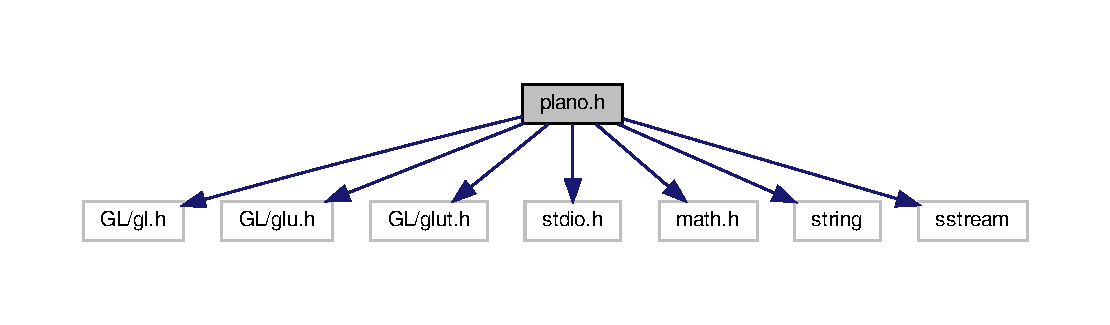
\includegraphics[width=350pt]{plano_8h__incl}
\end{center}
\end{figure}
Gráfico de los archivos que directa o indirectamente incluyen a este archivo\+:
\nopagebreak
\begin{figure}[H]
\begin{center}
\leavevmode
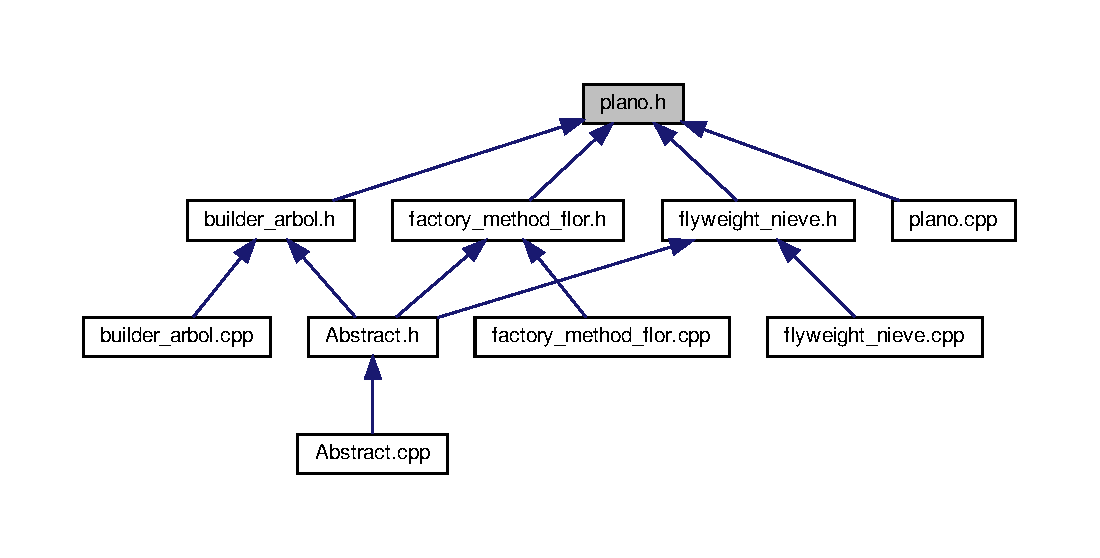
\includegraphics[width=350pt]{plano_8h__dep__incl}
\end{center}
\end{figure}
\subsection*{Clases}
\begin{DoxyCompactItemize}
\item 
struct \hyperlink{structcoordenada}{coordenada}
\item 
class \hyperlink{classplano}{plano}
\begin{DoxyCompactList}\small\item\em La clase plano tiene los elementos basicos para empezar a dibujar como se hace en la python turtle.  Definicion de la funciones usadas en la clase. \end{DoxyCompactList}\end{DoxyCompactItemize}
\subsection*{defines}
\begin{DoxyCompactItemize}
\item 
\mbox{\Hypertarget{plano_8h_a598a3330b3c21701223ee0ca14316eca}\label{plano_8h_a598a3330b3c21701223ee0ca14316eca}} 
\#define {\bfseries PI}~3.\+1415926535897932384626433832795
\end{DoxyCompactItemize}
\subsection*{typedefs}
\begin{DoxyCompactItemize}
\item 
\mbox{\Hypertarget{plano_8h_abce788b74b2513b814786f28fcdd11f7}\label{plano_8h_abce788b74b2513b814786f28fcdd11f7}} 
typedef double {\bfseries t\+\_\+coord}
\end{DoxyCompactItemize}


\subsection{Descripción detallada}
implementacion de clase plano que permite hacer dibujos usando open\+GL. 

\begin{DoxyAuthor}{Autor}
Walker Manrique 
\end{DoxyAuthor}
\begin{DoxyVersion}{Versión}
Revision 1.\+1 
\end{DoxyVersion}

%--- End generated contents ---

% Index
\backmatter
\newpage
\phantomsection
\clearemptydoublepage
\addcontentsline{toc}{chapter}{Índice}
\printindex

\end{document}
